\documentclass{beamer}

\mode<presentation> {

%\usetheme{default}
%\usetheme{AnnArbor}
%\usetheme{Antibes}
%\usetheme{Bergen}
%\usetheme{Berkeley}
%\usetheme{Berlin}
%\usetheme{Boadilla}
%\usetheme{CambridgeUS}
%\usetheme{Copenhagen}
%\usetheme{Darmstadt}
%\usetheme{Dresden}
%\usetheme{Frankfurt}
%\usetheme{Goettingen}
%\usetheme{Hannover}
%\usetheme{Ilmenau}
%\usetheme{JuanLesPins}
%\usetheme{Luebeck}
\usetheme{Madrid}
%\usetheme{Malmoe}
%\usetheme{Marburg}
%\usetheme{Montpellier}
%\usetheme{PaloAlto}
%\usetheme{Pittsburgh}
%\usetheme{Rochester}
%\usetheme{Singapore}
%\usetheme{Szeged}
%\usetheme{Warsaw}

%\usecolortheme{albatross}
%\usecolortheme{beaver}
%\usecolortheme{beetle}
%\usecolortheme{crane}
%\usecolortheme{dolphin}
%\usecolortheme{dove}
%\usecolortheme{fly}
%\usecolortheme{lily}
%\usecolortheme{orchid}
%\usecolortheme{rose}
%\usecolortheme{seagull}
%\usecolortheme{seahorse}
%\usecolortheme{whale}
%\usecolortheme{wolverine}

%\setbeamertemplate{footline} % To remove the footer line in all slides uncomment this line
%\setbeamertemplate{footline}[page number] % To replace the footer line in all slides with a simple slide count uncomment this line
%\setbeamertemplate{navigation symbols}{} % To remove the navigation symbols from the bottom of all slides uncomment this line
}

\usepackage{graphicx}
\usepackage{booktabs}
\usepackage{tikz}
\usepackage{scalefnt}
\usepackage{listings}
\usepackage{todonotes}
\usepackage{tabularx}
\usepackage{enumitem}
\usepackage{hyperref}
\usepackage{xcolor}

\setitemize{label=\usebeamerfont*{itemize item}
\usebeamercolor[fg]{itemize item}
\usebeamertemplate{itemize item}}

\definecolor{ao(english)}{rgb}{0.0, 0.5, 0.0}
\definecolor{aureolin}{rgb}{0.99, 0.93, 0.0}
\definecolor{bostonuniversityred}{rgb}{0.8, 0.0, 0.0}

\renewcommand{\tabularxcolumn}[1]{>{\small}m{#1}}
\renewcommand{\arraystretch}{2}

%% Listings definition for Go language
%% Go language reference : http://www.golang.org
%% Author : Uriel Corfa <uriel@corfa.fr>
%% Project home: https://bitbucket.org/korfuri/golang-latex-listings

\lstdefinelanguage{go}{
  % Keywords as defined in the BNF
  morekeywords=[1]{break,default,func,interface,%
    case,defer,go,map,struct,chan,else,goto,package,%
    switch,const,fallthrough,if,range,type,continue,%
    for,import,return,var,select},
  % Special identifiers, builtin functions
  morekeywords=[2]{make,new,nil,len,cap,copy,complex,%
    real,imag,panic,recover,print,println,iota,close,%
    closed,_,true,false,append,delete},
  % Basic types
  morekeywords=[3]{%
    string,int,uint,uintptr,double,float,byte,%
    int8,int16,int32,int64,int128,%
    uint8,uint16,uint32,uint64,uint128,%
    float32,float64,complex64,complex128,%
    rune},
  % Strings : "toto", 'toto', `toto`
  morestring=[b]{"},
  morestring=[b]{'},
  morestring=[b]{`},
  % Comments : /* comment */ and // comment
  comment=[l]{//},
  morecomment=[s]{/*}{*/},
  % Options
  sensitive=true
}

\lstset{
  language={go},
  basicstyle=\ttfamily\tiny
}

\title[ICS Honeypot]{Industrial Control Systems Honeypot}

\author{May1601}
\institute[]
{
Dan Borgerding \\
Jon Hope \\
Nik Kinkel \\
Jon Osborne \\
Korbin Stich \\
\medskip
\url{http://may1601.sd.ece.iastate.edu}

\textbf{Client}: Alliant Energy

\textbf{Advisor}: Dr. Doug Jacobson
}
\date{\today}

\begin{document}

\begin{titlepage}

\begin{center}

\textup{\small {\bf CPRE/EE/SE 491} \\ Senior Design}\\[0.2in]

% Title
\Large \textbf {May1601 Project Plan}\\[0.5in]

% Submitted by
\normalsize Submitted by \\
\begin{table}[h]
\centering
\begin{tabular}{lr}\hline \\
Jonathan Osborne & Team Leader \\
Nik Kinkel & Key Concept Holder \\ 
Korbin Stich & Key Concept Holder \\ 
Daniel Borgerding & Communication Leader \\ 
Jonathan Hope & Webmaster \\
\\ \hline
%Korbin Stich &  \\ \\ \hline 

\end{tabular}
\end{table}

\vspace{.3in}
Under the guidance of\\
{\textbf{Dr. Doug Jacobson}}\\[0.3in]

\vspace{.3in}
Prepared for\\
{\textbf{Alliant Energy}}\\[0.3in]

\vfill

% Bottom of the page
\vspace{0.2cm}
Fall 2015

\end{center}
\end{titlepage}

\begin{titlepage}
\begin{center}

\vspace*{\fill}
\Huge \textbf {Industrial Control System Honeypot and Traffic Monitor}\\[0.5in]
\vspace*{\fill}

\end{center}
\end{titlepage}

%\begin{frame}
\frametitle{Overview}
\tableofcontents
\end{frame}
 % <-- includes TOC
\section{Project Plan}

% Slide 1
\begin{frame}
\frametitle{Problem Statement}
The goal of the project is to create a standalone security device that can be placed in an industrial network to monitor traffic, looking for security-related deviations, and act as a low interaction honeypot.

\hfill

\textbf{Deliverable}
\begin{itemize}
\item Raspberry Pi (Raspbian)
\item Hardened System
\item Honeypot \& Logging Framework
\item Small, passive IDS
\item Automated deployment process
\end{itemize}

\end{frame}

% Slide 2
\begin{frame}
\frametitle{Conceptual Sketch}
\begin{figure}
\centering
{\scalefont{0.75}
\scalebox{0.7}{% Graphic for TeX using PGF
% Title: /home/nskinkel/src/may1601/docs/fall2015/project_plan/report/Diagram1.dia
% Creator: Dia v0.97.3
% CreationDate: Sat Oct  3 18:51:05 2015
% For: nskinkel
% \usepackage{tikz}
% The following commands are not supported in PSTricks at present
% We define them conditionally, so when they are implemented,
% this pgf file will use them.
\ifx\du\undefined
  \newlength{\du}
\fi
\setlength{\du}{15\unitlength}
\begin{tikzpicture}
\pgftransformxscale{0.600000}
\pgftransformyscale{-0.600000}
\definecolor{dialinecolor}{rgb}{0.000000, 0.000000, 0.000000}
\pgfsetstrokecolor{dialinecolor}
\definecolor{dialinecolor}{rgb}{1.000000, 1.000000, 1.000000}
\pgfsetfillcolor{dialinecolor}
\definecolor{dialinecolor}{rgb}{1.000000, 1.000000, 1.000000}
\pgfsetfillcolor{dialinecolor}
\fill (5.650000\du,3.300000\du)--(5.650000\du,25.950000\du)--(41.750000\du,25.950000\du)--(41.750000\du,3.300000\du)--cycle;
\pgfsetlinewidth{0.100000\du}
\pgfsetdash{}{0pt}
\pgfsetdash{}{0pt}
\pgfsetmiterjoin
\definecolor{dialinecolor}{rgb}{0.000000, 0.000000, 0.000000}
\pgfsetstrokecolor{dialinecolor}
\draw (5.650000\du,3.300000\du)--(5.650000\du,25.950000\du)--(41.750000\du,25.950000\du)--(41.750000\du,3.300000\du)--cycle;
% setfont left to latex
\definecolor{dialinecolor}{rgb}{0.000000, 0.000000, 0.000000}
\pgfsetstrokecolor{dialinecolor}
\node at (23.700000\du,14.820000\du){};
\definecolor{dialinecolor}{rgb}{1.000000, 1.000000, 1.000000}
\pgfsetfillcolor{dialinecolor}
\fill (9.925000\du,12.200000\du)--(9.925000\du,23.550000\du)--(16.500000\du,23.550000\du)--(16.500000\du,12.200000\du)--cycle;
\pgfsetlinewidth{0.100000\du}
\pgfsetdash{}{0pt}
\pgfsetdash{}{0pt}
\pgfsetmiterjoin
\definecolor{dialinecolor}{rgb}{0.000000, 0.000000, 0.000000}
\pgfsetstrokecolor{dialinecolor}
\draw (9.925000\du,12.200000\du)--(9.925000\du,23.550000\du)--(16.500000\du,23.550000\du)--(16.500000\du,12.200000\du)--cycle;
% setfont left to latex
\definecolor{dialinecolor}{rgb}{0.000000, 0.000000, 0.000000}
\pgfsetstrokecolor{dialinecolor}
\node at (13.212500\du,18.070000\du){};
\pgfsetlinewidth{0.200000\du}
\pgfsetdash{}{0pt}
\pgfsetdash{}{0pt}
\pgfsetbuttcap
{
\definecolor{dialinecolor}{rgb}{0.000000, 0.000000, 0.000000}
\pgfsetfillcolor{dialinecolor}
% was here!!!
\pgfsetarrowsend{latex}
\definecolor{dialinecolor}{rgb}{0.000000, 0.000000, 0.000000}
\pgfsetstrokecolor{dialinecolor}
\draw (2.000000\du,3.400000\du)--(1.991667\du,25.770833\du);
}
\pgfsetlinewidth{0.200000\du}
\pgfsetdash{}{0pt}
\pgfsetdash{}{0pt}
\pgfsetbuttcap
{
\definecolor{dialinecolor}{rgb}{0.000000, 0.000000, 0.000000}
\pgfsetfillcolor{dialinecolor}
% was here!!!
\pgfsetarrowsend{latex}
\definecolor{dialinecolor}{rgb}{0.000000, 0.000000, 0.000000}
\pgfsetstrokecolor{dialinecolor}
\draw (2.991667\du,25.904167\du)--(3.000000\du,3.350000\du);
}
\definecolor{dialinecolor}{rgb}{1.000000, 1.000000, 1.000000}
\pgfsetfillcolor{dialinecolor}
\fill (10.100000\du,4.200000\du)--(10.100000\du,7.650000\du)--(17.050000\du,7.650000\du)--(17.050000\du,4.200000\du)--cycle;
\pgfsetlinewidth{0.100000\du}
\pgfsetdash{}{0pt}
\pgfsetdash{}{0pt}
\pgfsetmiterjoin
\definecolor{dialinecolor}{rgb}{0.000000, 0.000000, 0.000000}
\pgfsetstrokecolor{dialinecolor}
\draw (10.100000\du,4.200000\du)--(10.100000\du,7.650000\du)--(17.050000\du,7.650000\du)--(17.050000\du,4.200000\du)--cycle;
% setfont left to latex
\definecolor{dialinecolor}{rgb}{0.000000, 0.000000, 0.000000}
\pgfsetstrokecolor{dialinecolor}
\node at (13.575000\du,6.120000\du){Bro IDS};
\pgfsetlinewidth{0.100000\du}
\pgfsetdash{}{0pt}
\pgfsetdash{}{0pt}
\pgfsetbuttcap
{
\definecolor{dialinecolor}{rgb}{0.000000, 0.000000, 0.000000}
\pgfsetfillcolor{dialinecolor}
% was here!!!
\pgfsetarrowsend{latex}
\definecolor{dialinecolor}{rgb}{0.000000, 0.000000, 0.000000}
\pgfsetstrokecolor{dialinecolor}
\draw (2.950000\du,6.000000\du)--(10.051059\du,5.949875\du);
}
\definecolor{dialinecolor}{rgb}{1.000000, 1.000000, 1.000000}
\pgfsetfillcolor{dialinecolor}
\fill (4.533333\du,6.305000\du)--(4.533333\du,10.250000\du)--(6.765833\du,10.250000\du)--(6.765833\du,6.305000\du)--cycle;
% setfont left to latex
\definecolor{dialinecolor}{rgb}{0.000000, 0.000000, 0.000000}
\pgfsetstrokecolor{dialinecolor}
\node[anchor=west] at (4.533333\du,6.900000\du){};
% setfont left to latex
\definecolor{dialinecolor}{rgb}{0.000000, 0.000000, 0.000000}
\pgfsetstrokecolor{dialinecolor}
\node[anchor=west] at (4.533333\du,7.700000\du){Sniffed};
% setfont left to latex
\definecolor{dialinecolor}{rgb}{0.000000, 0.000000, 0.000000}
\pgfsetstrokecolor{dialinecolor}
\node[anchor=west] at (4.533333\du,8.500000\du){Traffic};
% setfont left to latex
\definecolor{dialinecolor}{rgb}{0.000000, 0.000000, 0.000000}
\pgfsetstrokecolor{dialinecolor}
\node[anchor=west] at (4.533333\du,9.300000\du){};
% setfont left to latex
\definecolor{dialinecolor}{rgb}{0.000000, 0.000000, 0.000000}
\pgfsetstrokecolor{dialinecolor}
\node[anchor=west] at (4.533333\du,10.100000\du){};
\definecolor{dialinecolor}{rgb}{1.000000, 1.000000, 1.000000}
\pgfsetfillcolor{dialinecolor}
\fill (22.466667\du,11.591667\du)--(22.466667\du,14.291667\du)--(28.066667\du,14.291667\du)--(28.066667\du,11.591667\du)--cycle;
\pgfsetlinewidth{0.100000\du}
\pgfsetdash{}{0pt}
\pgfsetdash{}{0pt}
\pgfsetmiterjoin
\definecolor{dialinecolor}{rgb}{0.000000, 0.000000, 0.000000}
\pgfsetstrokecolor{dialinecolor}
\draw (22.466667\du,11.591667\du)--(22.466667\du,14.291667\du)--(28.066667\du,14.291667\du)--(28.066667\du,11.591667\du)--cycle;
% setfont left to latex
\definecolor{dialinecolor}{rgb}{0.000000, 0.000000, 0.000000}
\pgfsetstrokecolor{dialinecolor}
\node at (25.266667\du,12.736667\du){Microservice};
% setfont left to latex
\definecolor{dialinecolor}{rgb}{0.000000, 0.000000, 0.000000}
\pgfsetstrokecolor{dialinecolor}
\node at (25.266667\du,13.536667\du){Honeypot};
\definecolor{dialinecolor}{rgb}{1.000000, 1.000000, 1.000000}
\pgfsetfillcolor{dialinecolor}
\fill (22.555000\du,16.541667\du)--(22.555000\du,19.241667\du)--(28.155000\du,19.241667\du)--(28.155000\du,16.541667\du)--cycle;
\pgfsetlinewidth{0.100000\du}
\pgfsetdash{}{0pt}
\pgfsetdash{}{0pt}
\pgfsetmiterjoin
\definecolor{dialinecolor}{rgb}{0.000000, 0.000000, 0.000000}
\pgfsetstrokecolor{dialinecolor}
\draw (22.555000\du,16.541667\du)--(22.555000\du,19.241667\du)--(28.155000\du,19.241667\du)--(28.155000\du,16.541667\du)--cycle;
% setfont left to latex
\definecolor{dialinecolor}{rgb}{0.000000, 0.000000, 0.000000}
\pgfsetstrokecolor{dialinecolor}
\node at (25.355000\du,17.686667\du){Microservice};
% setfont left to latex
\definecolor{dialinecolor}{rgb}{0.000000, 0.000000, 0.000000}
\pgfsetstrokecolor{dialinecolor}
\node at (25.355000\du,18.486667\du){Honeypot};
\definecolor{dialinecolor}{rgb}{1.000000, 1.000000, 1.000000}
\pgfsetfillcolor{dialinecolor}
\fill (22.476667\du,21.450000\du)--(22.476667\du,24.150000\du)--(28.076667\du,24.150000\du)--(28.076667\du,21.450000\du)--cycle;
\pgfsetlinewidth{0.100000\du}
\pgfsetdash{}{0pt}
\pgfsetdash{}{0pt}
\pgfsetmiterjoin
\definecolor{dialinecolor}{rgb}{0.000000, 0.000000, 0.000000}
\pgfsetstrokecolor{dialinecolor}
\draw (22.476667\du,21.450000\du)--(22.476667\du,24.150000\du)--(28.076667\du,24.150000\du)--(28.076667\du,21.450000\du)--cycle;
% setfont left to latex
\definecolor{dialinecolor}{rgb}{0.000000, 0.000000, 0.000000}
\pgfsetstrokecolor{dialinecolor}
\node at (25.276667\du,22.595000\du){Microservice};
% setfont left to latex
\definecolor{dialinecolor}{rgb}{0.000000, 0.000000, 0.000000}
\pgfsetstrokecolor{dialinecolor}
\node at (25.276667\du,23.395000\du){Honeypot};
\pgfsetlinewidth{0.100000\du}
\pgfsetdash{}{0pt}
\pgfsetdash{}{0pt}
\pgfsetmiterjoin
\pgfsetbuttcap
{
\definecolor{dialinecolor}{rgb}{0.000000, 0.000000, 0.000000}
\pgfsetfillcolor{dialinecolor}
% was here!!!
\pgfsetarrowsend{latex}
{\pgfsetcornersarced{\pgfpoint{0.000000\du}{0.000000\du}}\definecolor{dialinecolor}{rgb}{0.000000, 0.000000, 0.000000}
\pgfsetstrokecolor{dialinecolor}
\draw (16.550407\du,17.875000\du)--(19.483363\du,17.875000\du)--(19.483363\du,12.941667\du)--(22.416319\du,12.941667\du);
}}
\pgfsetlinewidth{0.100000\du}
\pgfsetdash{}{0pt}
\pgfsetdash{}{0pt}
\pgfsetmiterjoin
\pgfsetbuttcap
{
\definecolor{dialinecolor}{rgb}{0.000000, 0.000000, 0.000000}
\pgfsetfillcolor{dialinecolor}
% was here!!!
\pgfsetarrowsend{latex}
{\pgfsetcornersarced{\pgfpoint{0.000000\du}{0.000000\du}}\definecolor{dialinecolor}{rgb}{0.000000, 0.000000, 0.000000}
\pgfsetstrokecolor{dialinecolor}
\draw (16.550407\du,17.875000\du)--(19.488363\du,17.875000\du)--(19.488363\du,22.800000\du)--(22.426319\du,22.800000\du);
}}
\pgfsetlinewidth{0.100000\du}
\pgfsetdash{}{0pt}
\pgfsetdash{}{0pt}
\pgfsetmiterjoin
\pgfsetbuttcap
{
\definecolor{dialinecolor}{rgb}{0.000000, 0.000000, 0.000000}
\pgfsetfillcolor{dialinecolor}
% was here!!!
\pgfsetarrowsend{latex}
{\pgfsetcornersarced{\pgfpoint{0.000000\du}{0.000000\du}}\definecolor{dialinecolor}{rgb}{0.000000, 0.000000, 0.000000}
\pgfsetstrokecolor{dialinecolor}
\draw (16.550407\du,17.875000\du)--(19.527530\du,17.875000\du)--(19.527530\du,17.891667\du)--(22.504652\du,17.891667\du);
}}
% setfont left to latex
\definecolor{dialinecolor}{rgb}{0.000000, 0.000000, 0.000000}
\pgfsetstrokecolor{dialinecolor}
\node[anchor=west] at (23.700000\du,14.625000\du){};
\definecolor{dialinecolor}{rgb}{1.000000, 1.000000, 1.000000}
\pgfsetfillcolor{dialinecolor}
\fill (34.250000\du,8.200000\du)--(34.250000\du,20.150000\du)--(40.500000\du,20.150000\du)--(40.500000\du,8.200000\du)--cycle;
\pgfsetlinewidth{0.100000\du}
\pgfsetdash{}{0pt}
\pgfsetdash{}{0pt}
\pgfsetmiterjoin
\definecolor{dialinecolor}{rgb}{0.000000, 0.000000, 0.000000}
\pgfsetstrokecolor{dialinecolor}
\draw (34.250000\du,8.200000\du)--(34.250000\du,20.150000\du)--(40.500000\du,20.150000\du)--(40.500000\du,8.200000\du)--cycle;
% setfont left to latex
\definecolor{dialinecolor}{rgb}{0.000000, 0.000000, 0.000000}
\pgfsetstrokecolor{dialinecolor}
\node at (37.375000\du,14.370000\du){Logger};
\pgfsetlinewidth{0.100000\du}
\pgfsetdash{}{0pt}
\pgfsetdash{}{0pt}
\pgfsetmiterjoin
\pgfsetbuttcap
{
\definecolor{dialinecolor}{rgb}{0.000000, 0.000000, 0.000000}
\pgfsetfillcolor{dialinecolor}
% was here!!!
\pgfsetarrowsend{latex}
{\pgfsetcornersarced{\pgfpoint{0.000000\du}{0.000000\du}}\definecolor{dialinecolor}{rgb}{0.000000, 0.000000, 0.000000}
\pgfsetstrokecolor{dialinecolor}
\draw (17.099456\du,5.925000\du)--(31.550000\du,5.925000\du)--(31.550000\du,14.175000\du)--(34.200119\du,14.175000\du);
}}
\pgfsetlinewidth{0.100000\du}
\pgfsetdash{}{0pt}
\pgfsetdash{}{0pt}
\pgfsetmiterjoin
\pgfsetbuttcap
{
\definecolor{dialinecolor}{rgb}{0.000000, 0.000000, 0.000000}
\pgfsetfillcolor{dialinecolor}
% was here!!!
\pgfsetarrowsend{latex}
{\pgfsetcornersarced{\pgfpoint{0.000000\du}{0.000000\du}}\definecolor{dialinecolor}{rgb}{0.000000, 0.000000, 0.000000}
\pgfsetstrokecolor{dialinecolor}
\draw (28.115336\du,12.941667\du)--(31.550000\du,12.941667\du)--(31.550000\du,14.175000\du)--(34.200119\du,14.175000\du);
}}
\pgfsetlinewidth{0.100000\du}
\pgfsetdash{}{0pt}
\pgfsetdash{}{0pt}
\pgfsetmiterjoin
\pgfsetbuttcap
{
\definecolor{dialinecolor}{rgb}{0.000000, 0.000000, 0.000000}
\pgfsetfillcolor{dialinecolor}
% was here!!!
\pgfsetarrowsend{latex}
{\pgfsetcornersarced{\pgfpoint{0.000000\du}{0.000000\du}}\definecolor{dialinecolor}{rgb}{0.000000, 0.000000, 0.000000}
\pgfsetstrokecolor{dialinecolor}
\draw (28.205214\du,17.891667\du)--(31.550000\du,17.891667\du)--(31.550000\du,14.175000\du)--(34.200119\du,14.175000\du);
}}
\pgfsetlinewidth{0.100000\du}
\pgfsetdash{}{0pt}
\pgfsetdash{}{0pt}
\pgfsetmiterjoin
\pgfsetbuttcap
{
\definecolor{dialinecolor}{rgb}{0.000000, 0.000000, 0.000000}
\pgfsetfillcolor{dialinecolor}
% was here!!!
\pgfsetarrowsend{latex}
{\pgfsetcornersarced{\pgfpoint{0.000000\du}{0.000000\du}}\definecolor{dialinecolor}{rgb}{0.000000, 0.000000, 0.000000}
\pgfsetstrokecolor{dialinecolor}
\draw (28.126163\du,22.800000\du)--(31.550000\du,22.800000\du)--(31.550000\du,14.175000\du)--(34.200119\du,14.175000\du);
}}
% setfont left to latex
\definecolor{dialinecolor}{rgb}{0.000000, 0.000000, 0.000000}
\pgfsetstrokecolor{dialinecolor}
\node[anchor=west] at (23.700000\du,14.625000\du){};
% setfont left to latex
\definecolor{dialinecolor}{rgb}{0.000000, 0.000000, 0.000000}
\pgfsetstrokecolor{dialinecolor}
\node[anchor=west] at (20.150000\du,4.933333\du){Alerts aggregated and formatted for Splunk};
% setfont left to latex
\definecolor{dialinecolor}{rgb}{0.000000, 0.000000, 0.000000}
\pgfsetstrokecolor{dialinecolor}
\node[anchor=west] at (12.716667\du,10.700000\du){Honeypot traffic forwarded};
% setfont left to latex
\definecolor{dialinecolor}{rgb}{0.000000, 0.000000, 0.000000}
\pgfsetstrokecolor{dialinecolor}
\node[anchor=west] at (12.716667\du,11.500000\du){    to localhost services};
% setfont left to latex
\definecolor{dialinecolor}{rgb}{0.000000, 0.000000, 0.000000}
\pgfsetstrokecolor{dialinecolor}
\node[anchor=west] at (10.858333\du,16.637500\du){};
% setfont left to latex
\definecolor{dialinecolor}{rgb}{0.000000, 0.000000, 0.000000}
\pgfsetstrokecolor{dialinecolor}
\node[anchor=west] at (10.858333\du,17.437500\du){  Public};
% setfont left to latex
\definecolor{dialinecolor}{rgb}{0.000000, 0.000000, 0.000000}
\pgfsetstrokecolor{dialinecolor}
\node[anchor=west] at (10.858333\du,18.237500\du){Interface};
% setfont left to latex
\definecolor{dialinecolor}{rgb}{0.000000, 0.000000, 0.000000}
\pgfsetstrokecolor{dialinecolor}
\node[anchor=west] at (10.858333\du,19.037500\du){};
\pgfsetlinewidth{0.100000\du}
\pgfsetdash{}{0pt}
\pgfsetdash{}{0pt}
\pgfsetbuttcap
{
\definecolor{dialinecolor}{rgb}{0.000000, 0.000000, 0.000000}
\pgfsetfillcolor{dialinecolor}
% was here!!!
\pgfsetarrowsend{latex}
\definecolor{dialinecolor}{rgb}{0.000000, 0.000000, 0.000000}
\pgfsetstrokecolor{dialinecolor}
\draw (2.991667\du,17.837500\du)--(9.874697\du,17.862754\du);
}
\definecolor{dialinecolor}{rgb}{1.000000, 1.000000, 1.000000}
\pgfsetfillcolor{dialinecolor}
\fill (4.125000\du,17.909167\du)--(4.125000\du,21.054167\du)--(7.077500\du,21.054167\du)--(7.077500\du,17.909167\du)--cycle;
% setfont left to latex
\definecolor{dialinecolor}{rgb}{0.000000, 0.000000, 0.000000}
\pgfsetstrokecolor{dialinecolor}
\node[anchor=west] at (4.125000\du,18.504167\du){};
% setfont left to latex
\definecolor{dialinecolor}{rgb}{0.000000, 0.000000, 0.000000}
\pgfsetstrokecolor{dialinecolor}
\node[anchor=west] at (4.125000\du,19.304167\du){Incoming};
% setfont left to latex
\definecolor{dialinecolor}{rgb}{0.000000, 0.000000, 0.000000}
\pgfsetstrokecolor{dialinecolor}
\node[anchor=west] at (4.125000\du,20.104167\du){  Traffic};
% setfont left to latex
\definecolor{dialinecolor}{rgb}{0.000000, 0.000000, 0.000000}
\pgfsetstrokecolor{dialinecolor}
\node[anchor=west] at (4.125000\du,20.904167\du){};
\pgfsetlinewidth{0.100000\du}
\pgfsetdash{}{0pt}
\pgfsetdash{}{0pt}
\pgfsetmiterjoin
\pgfsetbuttcap
{
\definecolor{dialinecolor}{rgb}{0.000000, 0.000000, 0.000000}
\pgfsetfillcolor{dialinecolor}
% was here!!!
\pgfsetarrowsend{latex}
{\pgfsetcornersarced{\pgfpoint{0.000000\du}{0.000000\du}}\definecolor{dialinecolor}{rgb}{0.000000, 0.000000, 0.000000}
\pgfsetstrokecolor{dialinecolor}
\draw (6.433182\du,17.850127\du)--(6.433182\du,9.770833\du)--(13.575000\du,9.770833\du)--(13.575000\du,7.700036\du);
}}
% setfont left to latex
\definecolor{dialinecolor}{rgb}{0.000000, 0.000000, 0.000000}
\pgfsetstrokecolor{dialinecolor}
\node[anchor=west] at (1.258333\du,0.637500\du){};
% setfont left to latex
\definecolor{dialinecolor}{rgb}{0.000000, 0.000000, 0.000000}
\pgfsetstrokecolor{dialinecolor}
\node[anchor=west] at (1.258333\du,1.437500\du){Network};
% setfont left to latex
\definecolor{dialinecolor}{rgb}{0.000000, 0.000000, 0.000000}
\pgfsetstrokecolor{dialinecolor}
\node[anchor=west] at (1.258333\du,2.237500\du){ Traffic};
\pgfsetlinewidth{0.100000\du}
\pgfsetdash{}{0pt}
\pgfsetdash{}{0pt}
\pgfsetbuttcap
{
\definecolor{dialinecolor}{rgb}{0.000000, 0.000000, 0.000000}
\pgfsetfillcolor{dialinecolor}
% was here!!!
\pgfsetarrowsend{latex}
\definecolor{dialinecolor}{rgb}{0.000000, 0.000000, 0.000000}
\pgfsetstrokecolor{dialinecolor}
\draw (40.548572\du,14.173477\du)--(46.058333\du,14.170833\du);
}
\definecolor{dialinecolor}{rgb}{1.000000, 1.000000, 1.000000}
\pgfsetfillcolor{dialinecolor}
\fill (40.658333\du,11.575833\du)--(40.658333\du,13.920833\du)--(43.708333\du,13.920833\du)--(43.708333\du,11.575833\du)--cycle;
% setfont left to latex
\definecolor{dialinecolor}{rgb}{0.000000, 0.000000, 0.000000}
\pgfsetstrokecolor{dialinecolor}
\node[anchor=west] at (40.658333\du,12.170833\du){};
% setfont left to latex
\definecolor{dialinecolor}{rgb}{0.000000, 0.000000, 0.000000}
\pgfsetstrokecolor{dialinecolor}
\node[anchor=west] at (40.658333\du,12.970833\du){To Splunk};
% setfont left to latex
\definecolor{dialinecolor}{rgb}{0.000000, 0.000000, 0.000000}
\pgfsetstrokecolor{dialinecolor}
\node[anchor=west] at (40.658333\du,13.770833\du){};
\end{tikzpicture}
}
}
\caption{Simplified Device Internals}
\end{figure}
\end{frame}

% Slide 3
\begin{frame}
\frametitle{Functional Requirements}
System Behavior
\begin{itemize}
\item Provide SSH, HTTP, HTTPS and necessary SCADA protocols 
\item A minimized passive intrusion detection system
\item Log attempted intrusion attempts and alert necessary personnel 
\item Automatic deployment and remote management
\item Easily customizable protocols
\end{itemize}

\end{frame}

% Slide 4
\begin{frame}
\frametitle{Non-functional Requirements}
System Performance
\begin{itemize}
\item Secure system design
\item Environmental considerations
\item System must be low maintenance
\item Simple stand alone device
\item Capable of expansion beyond scope of project
\end{itemize}

\end{frame}

% Slide 5
\begin{frame}
\frametitle{Technical/Other Constraints and Considerations}

\begin{itemize}
\item ARM architecture
\item Work with Alliant's existing logging architecture
\item Limited RAM provided by hardware
\item Unclear SCADA protocols
\item Dealing with sensitive information
\end{itemize}

\end{frame}

% Slide 6
\begin{frame}
\frametitle{Market Survey}
\begin{center}
\textbf{Open Source Honeypots}
\begin{tabular}{l | l}
\toprule
\textbf{ConPot} & \textbf{Kippo} \\
\midrule
Low Interaction & Medium Interaction \\
Siemens s7-200 PLC & Fake file system \\
MODBUS, HTTP, SNMP, s7comm & SSH \\
\bottomrule
\end{tabular}
\end{center}

\end{frame}

% Slide 7
\begin{frame}
\frametitle{Potential Risks \& Mitigation}

\huge Potential Risks \medskip
\normalsize
\begin{itemize}
    \item ESD, RFI, EMI.
    \item Ethernet Cable
    \item Physical Ingress Protection
    \item Limited Memory
    \item Security Concerns
\end{itemize}

\end{frame}

% Slide 8
\begin{frame}
\frametitle{Resource Cost Estimate}

\begin{center}

\begin{tabular}{l | l}
\toprule
\textbf{Item} & \textbf{Price} \\
\midrule
Raspberry PI B+ & \$69.99 (plus tax) \\
USB 3.0 Gigabit Ethernet Adapter & \$16.99 (plus tax) \\
\bottomrule
\end{tabular}

\hfill \break
\textbf{Total Cost: \$89.98 (plus tax)}
\end{center}


\end{frame}

\section{System Design}

% Slide 10
\begin{frame}
\frametitle{Functional Decomposition}

\begin{tabular}{l | l}
\toprule
\textbf{Component} & \textbf{Function} \\
\midrule
Honeypot Plugin Framework & Core, extensible interfaces \\
Default Plugin Set & Client-specific functionality \\
Automated Deployment System & Flexible rollouts/updates \\
Device & Components installed on device(s) \\
\bottomrule
\end{tabular}

\end{frame}

% Slide 11
\begin{frame}
\frametitle{Detailed Design: Honeypot Framework}

\begin{figure}
\centering
\caption{Plugin Framework Architecture}
{\scalefont{0.70}
\scalebox{0.7}{% Graphic for TeX using PGF
% Title: /home/nskinkel/plugins.dia
% Creator: Dia v0.97.3
% CreationDate: Sun Dec  6 18:02:21 2015
% For: nskinkel
% \usepackage{tikz}
% The following commands are not supported in PSTricks at present
% We define them conditionally, so when they are implemented,
% this pgf file will use them.
\ifx\du\undefined
  \newlength{\du}
\fi
\setlength{\du}{15\unitlength}
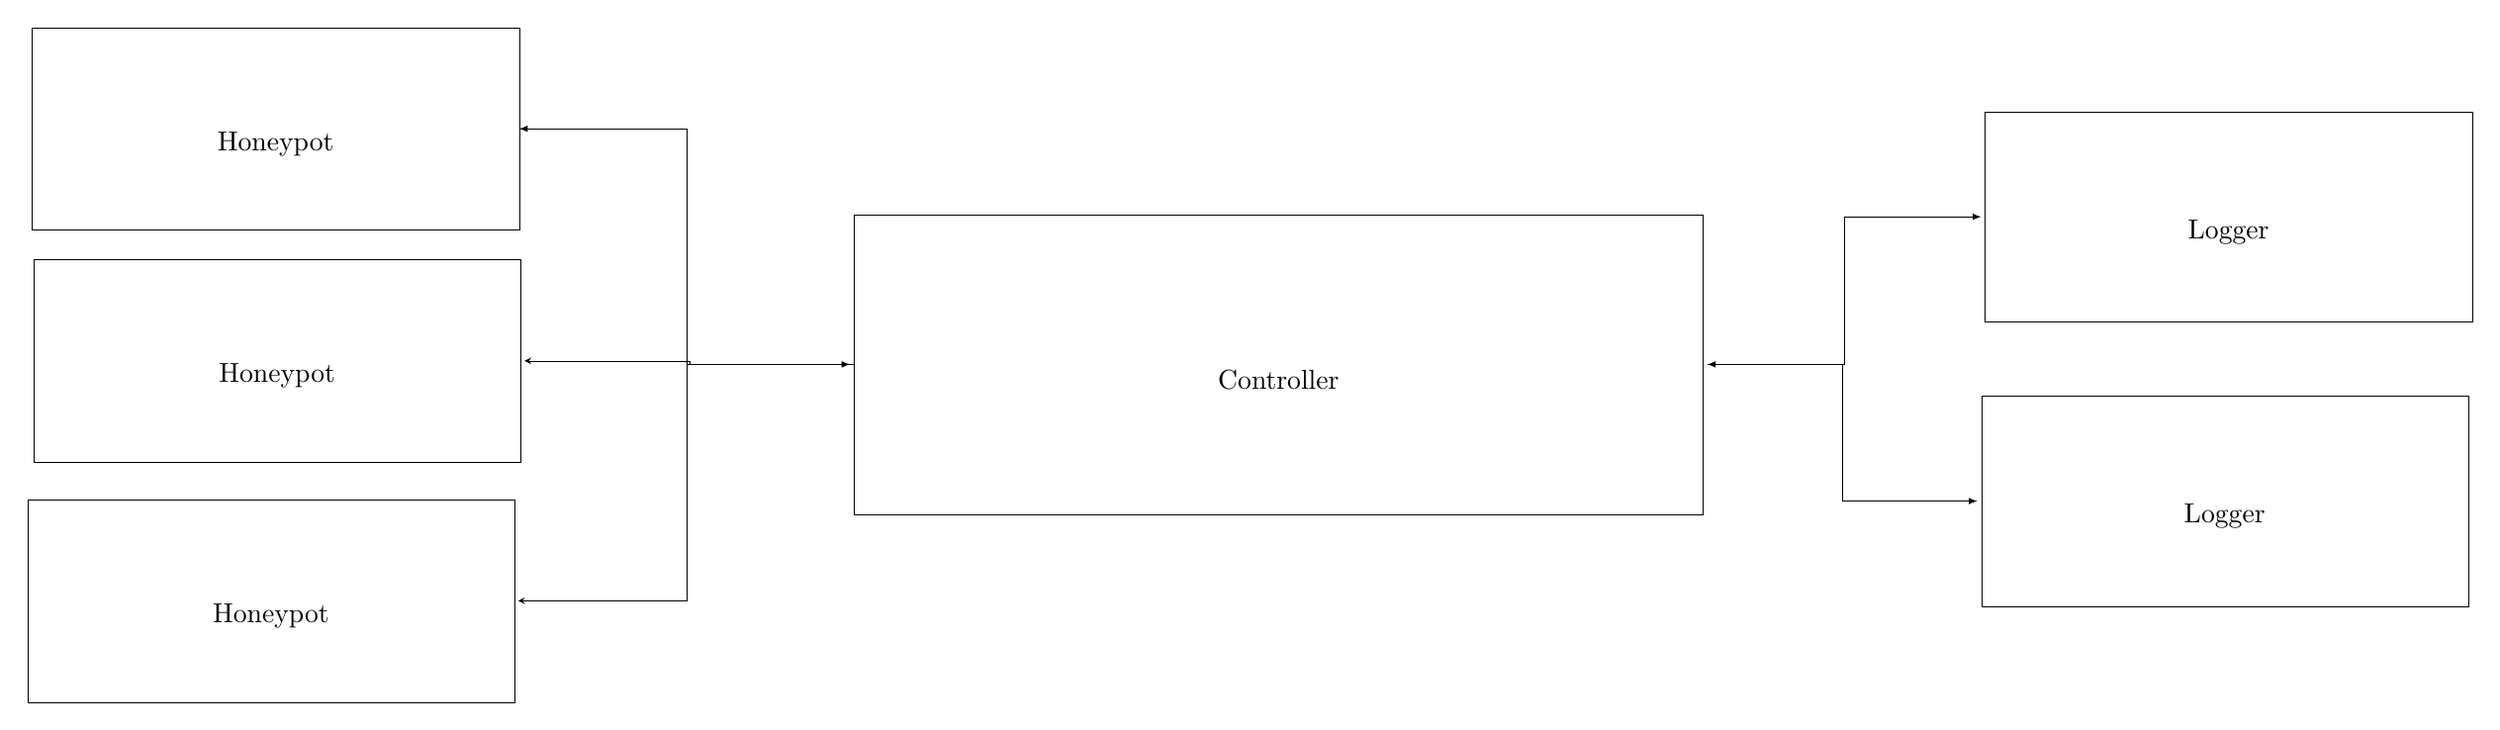
\begin{tikzpicture}
\pgftransformxscale{1.000000}
\pgftransformyscale{-1.000000}
\definecolor{dialinecolor}{rgb}{0.000000, 0.000000, 0.000000}
\pgfsetstrokecolor{dialinecolor}
\definecolor{dialinecolor}{rgb}{1.000000, 1.000000, 1.000000}
\pgfsetfillcolor{dialinecolor}
\definecolor{dialinecolor}{rgb}{1.000000, 1.000000, 1.000000}
\pgfsetfillcolor{dialinecolor}
\fill (6.250000\du,0.500000\du)--(6.250000\du,3.100000\du)--(12.500000\du,3.100000\du)--(12.500000\du,0.500000\du)--cycle;
\pgfsetlinewidth{0.100000\du}
\pgfsetdash{}{0pt}
\pgfsetdash{}{0pt}
\pgfsetmiterjoin
\definecolor{dialinecolor}{rgb}{0.000000, 0.000000, 0.000000}
\pgfsetstrokecolor{dialinecolor}
\draw (6.250000\du,0.500000\du)--(6.250000\du,3.100000\du)--(12.500000\du,3.100000\du)--(12.500000\du,0.500000\du)--cycle;
% setfont left to latex
\definecolor{dialinecolor}{rgb}{0.000000, 0.000000, 0.000000}
\pgfsetstrokecolor{dialinecolor}
\node at (9.375000\du,1.995000\du){Honeypot};
\definecolor{dialinecolor}{rgb}{1.000000, 1.000000, 1.000000}
\pgfsetfillcolor{dialinecolor}
\fill (6.270000\du,3.480000\du)--(6.270000\du,6.080000\du)--(12.520000\du,6.080000\du)--(12.520000\du,3.480000\du)--cycle;
\pgfsetlinewidth{0.100000\du}
\pgfsetdash{}{0pt}
\pgfsetdash{}{0pt}
\pgfsetmiterjoin
\definecolor{dialinecolor}{rgb}{0.000000, 0.000000, 0.000000}
\pgfsetstrokecolor{dialinecolor}
\draw (6.270000\du,3.480000\du)--(6.270000\du,6.080000\du)--(12.520000\du,6.080000\du)--(12.520000\du,3.480000\du)--cycle;
% setfont left to latex
\definecolor{dialinecolor}{rgb}{0.000000, 0.000000, 0.000000}
\pgfsetstrokecolor{dialinecolor}
\node at (9.395000\du,4.975000\du){Honeypot};
\definecolor{dialinecolor}{rgb}{1.000000, 1.000000, 1.000000}
\pgfsetfillcolor{dialinecolor}
\fill (6.190000\du,6.560000\du)--(6.190000\du,9.160000\du)--(12.440000\du,9.160000\du)--(12.440000\du,6.560000\du)--cycle;
\pgfsetlinewidth{0.100000\du}
\pgfsetdash{}{0pt}
\pgfsetdash{}{0pt}
\pgfsetmiterjoin
\definecolor{dialinecolor}{rgb}{0.000000, 0.000000, 0.000000}
\pgfsetstrokecolor{dialinecolor}
\draw (6.190000\du,6.560000\du)--(6.190000\du,9.160000\du)--(12.440000\du,9.160000\du)--(12.440000\du,6.560000\du)--cycle;
% setfont left to latex
\definecolor{dialinecolor}{rgb}{0.000000, 0.000000, 0.000000}
\pgfsetstrokecolor{dialinecolor}
\node at (9.315000\du,8.055000\du){Honeypot};
\definecolor{dialinecolor}{rgb}{1.000000, 1.000000, 1.000000}
\pgfsetfillcolor{dialinecolor}
\fill (31.320000\du,1.580000\du)--(31.320000\du,4.280000\du)--(37.570000\du,4.280000\du)--(37.570000\du,1.580000\du)--cycle;
\pgfsetlinewidth{0.100000\du}
\pgfsetdash{}{0pt}
\pgfsetdash{}{0pt}
\pgfsetmiterjoin
\definecolor{dialinecolor}{rgb}{0.000000, 0.000000, 0.000000}
\pgfsetstrokecolor{dialinecolor}
\draw (31.320000\du,1.580000\du)--(31.320000\du,4.280000\du)--(37.570000\du,4.280000\du)--(37.570000\du,1.580000\du)--cycle;
% setfont left to latex
\definecolor{dialinecolor}{rgb}{0.000000, 0.000000, 0.000000}
\pgfsetstrokecolor{dialinecolor}
\node at (34.445000\du,3.125000\du){Logger};
\definecolor{dialinecolor}{rgb}{1.000000, 1.000000, 1.000000}
\pgfsetfillcolor{dialinecolor}
\fill (31.270000\du,5.230000\du)--(31.270000\du,7.930000\du)--(37.520000\du,7.930000\du)--(37.520000\du,5.230000\du)--cycle;
\pgfsetlinewidth{0.100000\du}
\pgfsetdash{}{0pt}
\pgfsetdash{}{0pt}
\pgfsetmiterjoin
\definecolor{dialinecolor}{rgb}{0.000000, 0.000000, 0.000000}
\pgfsetstrokecolor{dialinecolor}
\draw (31.270000\du,5.230000\du)--(31.270000\du,7.930000\du)--(37.520000\du,7.930000\du)--(37.520000\du,5.230000\du)--cycle;
% setfont left to latex
\definecolor{dialinecolor}{rgb}{0.000000, 0.000000, 0.000000}
\pgfsetstrokecolor{dialinecolor}
\node at (34.395000\du,6.775000\du){Logger};
\definecolor{dialinecolor}{rgb}{1.000000, 1.000000, 1.000000}
\pgfsetfillcolor{dialinecolor}
\fill (16.800000\du,2.900000\du)--(16.800000\du,6.750000\du)--(27.700000\du,6.750000\du)--(27.700000\du,2.900000\du)--cycle;
\pgfsetlinewidth{0.100000\du}
\pgfsetdash{}{0pt}
\pgfsetdash{}{0pt}
\pgfsetmiterjoin
\definecolor{dialinecolor}{rgb}{0.000000, 0.000000, 0.000000}
\pgfsetstrokecolor{dialinecolor}
\draw (16.800000\du,2.900000\du)--(16.800000\du,6.750000\du)--(27.700000\du,6.750000\du)--(27.700000\du,2.900000\du)--cycle;
% setfont left to latex
\definecolor{dialinecolor}{rgb}{0.000000, 0.000000, 0.000000}
\pgfsetstrokecolor{dialinecolor}
\node at (22.250000\du,5.020000\du){Controller};
\pgfsetlinewidth{0.100000\du}
\pgfsetdash{}{0pt}
\pgfsetdash{}{0pt}
\pgfsetmiterjoin
\pgfsetbuttcap
{
\definecolor{dialinecolor}{rgb}{0.000000, 0.000000, 0.000000}
\pgfsetfillcolor{dialinecolor}
% was here!!!
\pgfsetarrowsstart{latex}
{\pgfsetcornersarced{\pgfpoint{0.000000\du}{0.000000\du}}\definecolor{dialinecolor}{rgb}{0.000000, 0.000000, 0.000000}
\pgfsetstrokecolor{dialinecolor}
\draw (12.500000\du,1.800000\du)--(14.650000\du,1.800000\du)--(14.650000\du,4.825000\du)--(16.800000\du,4.825000\du);
}}
\pgfsetlinewidth{0.100000\du}
\pgfsetdash{}{0pt}
\pgfsetdash{}{0pt}
\pgfsetmiterjoin
\pgfsetbuttcap
{
\definecolor{dialinecolor}{rgb}{0.000000, 0.000000, 0.000000}
\pgfsetfillcolor{dialinecolor}
% was here!!!
\pgfsetarrowsstart{stealth}
{\pgfsetcornersarced{\pgfpoint{0.000000\du}{0.000000\du}}\definecolor{dialinecolor}{rgb}{0.000000, 0.000000, 0.000000}
\pgfsetstrokecolor{dialinecolor}
\draw (12.570388\du,4.780000\du)--(14.685194\du,4.780000\du)--(14.685194\du,4.825000\du)--(16.800000\du,4.825000\du);
}}
\pgfsetlinewidth{0.100000\du}
\pgfsetdash{}{0pt}
\pgfsetdash{}{0pt}
\pgfsetmiterjoin
\pgfsetbuttcap
{
\definecolor{dialinecolor}{rgb}{0.000000, 0.000000, 0.000000}
\pgfsetfillcolor{dialinecolor}
% was here!!!
\pgfsetarrowsstart{stealth}
\pgfsetarrowsend{latex}
{\pgfsetcornersarced{\pgfpoint{0.000000\du}{0.000000\du}}\definecolor{dialinecolor}{rgb}{0.000000, 0.000000, 0.000000}
\pgfsetstrokecolor{dialinecolor}
\draw (12.489169\du,7.860000\du)--(14.650000\du,7.860000\du)--(14.650000\du,4.825000\du)--(16.749927\du,4.825000\du);
}}
\pgfsetlinewidth{0.100000\du}
\pgfsetdash{}{0pt}
\pgfsetdash{}{0pt}
\pgfsetmiterjoin
\pgfsetbuttcap
{
\definecolor{dialinecolor}{rgb}{0.000000, 0.000000, 0.000000}
\pgfsetfillcolor{dialinecolor}
% was here!!!
\pgfsetarrowsend{latex}
{\pgfsetcornersarced{\pgfpoint{0.000000\du}{0.000000\du}}\definecolor{dialinecolor}{rgb}{0.000000, 0.000000, 0.000000}
\pgfsetstrokecolor{dialinecolor}
\draw (27.750336\du,4.825000\du)--(29.484974\du,4.825000\du)--(29.484974\du,6.580000\du)--(31.219612\du,6.580000\du);
}}
\pgfsetlinewidth{0.100000\du}
\pgfsetdash{}{0pt}
\pgfsetdash{}{0pt}
\pgfsetmiterjoin
\pgfsetbuttcap
{
\definecolor{dialinecolor}{rgb}{0.000000, 0.000000, 0.000000}
\pgfsetfillcolor{dialinecolor}
% was here!!!
\pgfsetarrowsstart{latex}
\pgfsetarrowsend{latex}
{\pgfsetcornersarced{\pgfpoint{0.000000\du}{0.000000\du}}\definecolor{dialinecolor}{rgb}{0.000000, 0.000000, 0.000000}
\pgfsetstrokecolor{dialinecolor}
\draw (27.750336\du,4.825000\du)--(29.509974\du,4.825000\du)--(29.509974\du,2.930000\du)--(31.269612\du,2.930000\du);
}}
\end{tikzpicture}
}
}
\end{figure}

\begin{table}
\centering
\small
\begin{tabularx}{\linewidth}{X X}
\textbf{Modular, Extensible} & \textbf{Secure by Design} \\
\midrule
\begin{itemize}[leftmargin=-0.3mm,after=\vspace{-\baselineskip},noitemsep,nolistsep]
    \item 2 plugin types: Honeypot \& Logger
    \item Communicate via lo unix socket RPC
\end{itemize}
&
\begin{itemize}[leftmargin=-0.3mm,after=\vspace{-\baselineskip},noitemsep,nolistsep]
    \item Isolated, non-privileged processes
    \item Minimal protocol functionality
\end{itemize} \\
\end{tabularx}
\end{table}
\end{frame}

% Slide 12
\begin{frame}
\frametitle{Technology Platform}
\textbf{CanaKit Raspberry PI}
\begin{itemize}
\item Quad-Core 900 MHz Processor
\item 1GB Ram
\item Rasbian OS
\end{itemize}

\textbf{Software}
\begin{itemize}
\item Ansible (Provisioning)
\item Vagrant (Provisioned Testing)
\item Golang (Google Programming Language)
\end{itemize}


\end{frame}

% Slide 13
\begin{frame}

\frametitle{Test Plan}
\textbf{GoLang}

Integration testing can be completed by combining multiple unit tests into a larger framework with the "testing" package. 
What about multiple configurations or platforms though?\\~\\

\textbf {Vagrant} allows for easy replication of test environments through virtual machines. This provides a method for plugin end-end testing for any device setup. \\~\\

Vagrant allows for \textbf{Provisioning}. This means that a newly created VM can be give startup tasks that will run as an automated script.

\end{frame}

% Slide 13.1
\begin{frame}[fragile]
\frametitle{Test Plan Continued}
\begin{itemize} % Elaborate on each item
	\item Time complexity analysis
	\item Code output verification
	\end{itemize}

\begin{example}[Benchmark Code] % Explain Code & Elaborate on output testing
\begin{verbatim}
	func BenchmarkSplunk (b *testing.B){
		m := map[string]string{"username":"user","password":"pass"}
		http:=Http{Method:"POST",Path:"index.html",Parameters:m}
		ev := Event{...,Http: &http}
		for i := 0 ; i< b.N; i++{
			ev.Send();
		}
	}
\end{verbatim}
\end{example}
	\textbf{Output}
	BenchmarkSplunk    10000000    282 ns/op


\end{frame}

% Slide 14
\begin{frame}
\frametitle{Prototype Implementation}

\begin{table}
\centering
\small
\begin{tabularx}{\linewidth}{c X X}
\toprule
\textbf{Component} & \textbf{Code} & \textbf{Status} \\
\midrule
Default Plugin Set & \begin{itemize}[leftmargin=-0.3mm,after=\vspace{-\baselineskip},noitemsep,nolistsep]
                         \item[] \href{https://github.com/Senior-Design-May1601/webauth}{HTTP}
                         \item[] \href{https://github.com/Senior-Design-May1601/webauth}{HTTPS}
                         \item[] \href{https://github.com/Senior-Design-May1601/fssh}{SSH}
                         \item[] \href{https://github.com/Senior-Design-May1601/Splunk}{Splunk Logger}
                     \end{itemize} &
                    \begin{itemize}[leftmargin=-0.3mm,after=\vspace{-\baselineskip},noitemsep,nolistsep]
                         \item[] \textcolor{ao(english)}{Done}
                         \item[] \textcolor{ao(english)}{Done}
                         \item[] \textcolor{ao(english)}{Done}
                         \item[] \textcolor{ao(english)}{Done}
                     \end{itemize} \\ \hline
Auto Deployment and Provisioning & \href{https://github.com/Senior-Design-May1601/config}{Ansible playbooks} & \textcolor{ao(english)}{Done} \\ \hline
Plugin Core & \href{https://github.com/Senior-Design-May1601/projectmain}{Framework} & \textcolor{aureolin}{Work-in-progress} \\ \hline
Physical Install & N/A & \textcolor{bostonuniversityred}{TODO} \\ \hline
Testing & N/A & \textcolor{bostonuniversityred}{TODO} \\
\bottomrule
\end{tabularx}
\end{table}
\end{frame}

\section{Conclusion}

% Slide 15
\begin{frame}
\frametitle{Current Project Status}

% TODO

\end{frame}

% Slide 16
\begin{frame}
\frametitle{Team Task Responsibilities}

% TODO

\end{frame}


% Slide 17
\begin{frame}
\frametitle{Plan for Next Semester}

% TODO

\end{frame}

\section{Questions}

\begin{frame}
\Huge{\centerline{Questions}}
\end{frame}


\end{document} 
